\begin{prob}[1]\textbf{Gradient Descent Method}\\
\end{prob}
OBJECTIVE FUNCTION:
\[
\mbox{\textit{minimize }} f(x) = \dfrac{1}{2}x^{T}Qx + q x
\]
  where $Q$ is an $n \times n$ positive definite matrix, and it is not
  necessarily a diagonal matrix. Note that the solution to this problem
  is $x^{*} = -Q^{-1}q$. As an alternative, design a gradient descent
  algorithm that will solve this unconstrained problem. Please pay attention
  to the following:
  with variable $x \in \mathbf{R}$\\

GRADIENT OF OBJECTIVE FUNCTION
\begin{eqnarray*}
\nabla f(x) &= \dfrac{\partial f(x)}{\partial x_{i}} \forall i = 1,2,\ldots,n\\
 &= Qx + q
\end{eqnarray*}

HESSIAN OF OBJECTIVE FUNCTION
\begin{eqnarray*}
\nabla^{2} f(x) &= \dfrac{\partial^{2} f(x)}{\partial x_{i}^{2}} \forall i = 1,2,\ldots,n\\
 &= Q
\end{eqnarray*}



(b)Generate figures that look like Fig 9.6 in the textbook with different starting points.
  \begin{figure}[h!]
  \centering
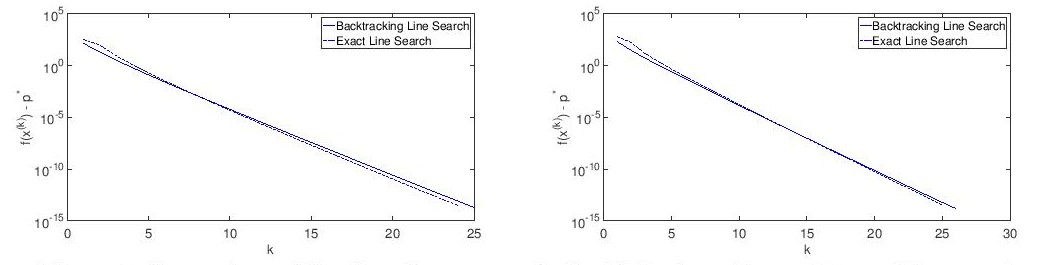
\includegraphics[width=\textwidth]{source/prob1/figu1}
%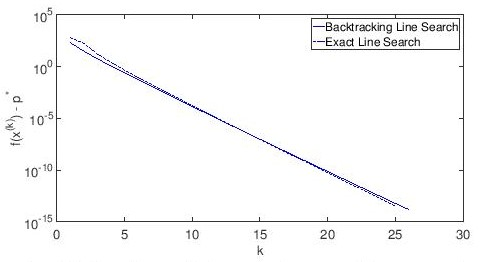
\includegraphics[width=5cm]{source/prob1/fig2}
\caption{Comparison of Gradient Descent with Backtracking and Exact Line Search for different starting points.}
\end{figure}

(c) Discuss the effects of different $\alpha$ and $\beta$ on the convergence of the Gradient Descent method with Backtracking Line search.\\

\begin{figure}[h!]
  \centering
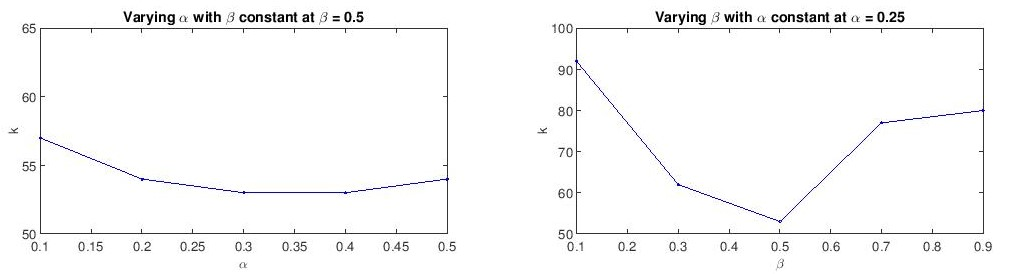
\includegraphics[width=\textwidth]{source/prob1/figu2}
%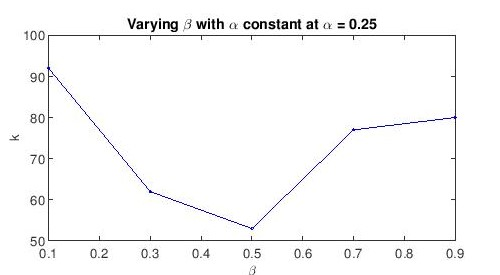
\includegraphics[width=5cm]{source/prob1/fig4}
\caption{Comparison of the convergence of Backtracking line search with varying $\alpha$ and $\beta$}
\end{figure}


(d) Investigate the effect of problem size $n$ on the convergence behavior of your algorithm\\

  \begin{figure}[H]
  \centering
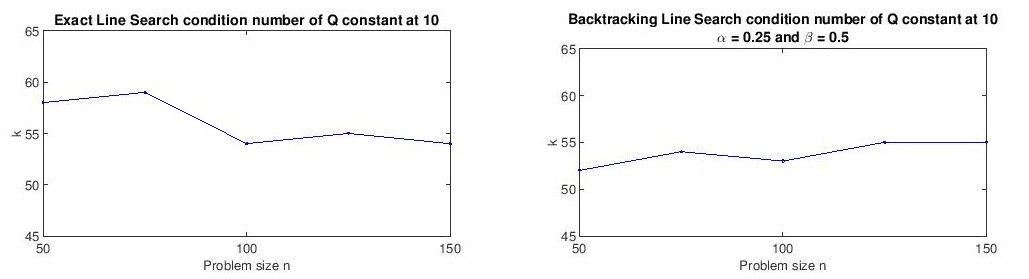
\includegraphics[width=\textwidth]{source/prob1/figu3}
%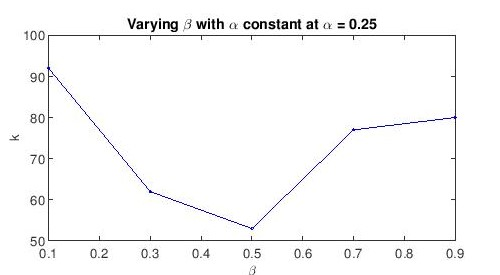
\includegraphics[width=5cm]{source/prob1/fig4}
\caption{Comparison of the convergence of the convergence of the Gradient Descent method by varying problem size $n$}
\end{figure}

(e) Investigate the effect of the condition number of $Q$ on the convergence behavior of your algorithm\\

  \begin{figure}[H]
  \centering
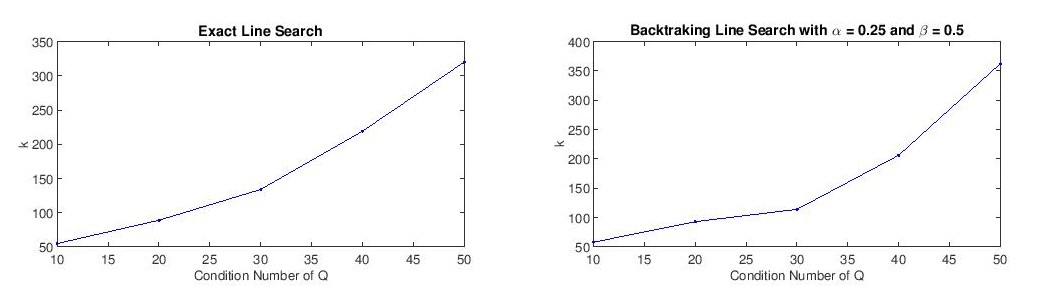
\includegraphics[width=\textwidth]{source/prob1/figu4}
%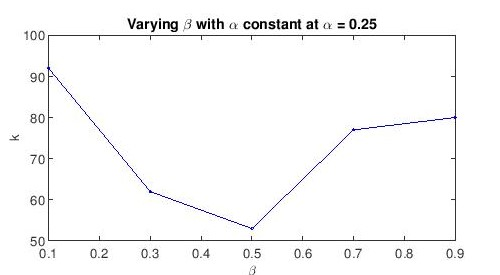
\includegraphics[width=5cm]{source/prob1/fig4}
\caption{Comparison of the convergence of the Gradient Descent method by varying the condition number of $Q$}
\end{figure}

(f)Design a steepest descent algorithm with the choice of norm is given as given at the bottom of pp. 476 of our textbook, where $P$ is selected as a diagonal matrix, whose diagonal elements are the
    same as those of $Q$. Is this new algorithm as sensitive to the condition number of $Q$?
    \begin{figure}[H]
  \centering
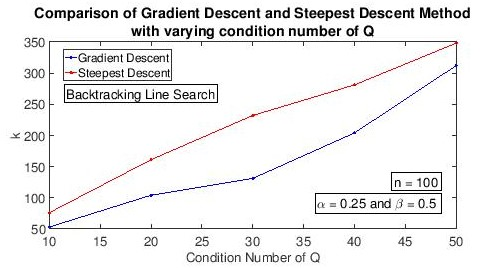
\includegraphics[width=7cm]{source/prob1/fig9}
%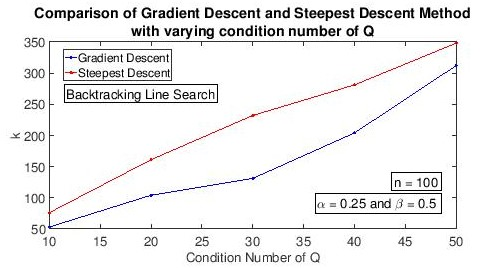
\includegraphics[width=5cm]{source/prob1/fig9}
\caption{Comparison of the convergence of the Gradient Descent method and the Steepest Descent method varying the condition number of $Q$}
\end{figure}  

(g) Comment on how the gradient descent algorithm can be used to
    solve a least-squares problem and give an example of a least-square
    problem tha tyou solve with this algorithm. Also, comment on the
    computational advantages of using the gradient descent algorithm
    as compared with just solving the linear system of equations
    $x^{*} = -Q q$. Do these advantages remain when the steepest descent
    approach described above is used? What are some potential disadvantages
    to using gradient descent, or steepest descent as compared with just
    solving the linear system of equations?
    
    The least-squares problem is a special case of the quadratic minimization problem:
    \[
    \mbox{minimize } \vert \vert Ax - b \vert \vert^{2}_{2} = x^{T} (A^{T} A)x - 2(A^{T}b)^{T} x + b^{T}b
    \]
    The optimality conditions for the least square problem is $A^{T} A x^{*} = A^{T}b$.
    The gradient descent is a faster method of solving a system of linear equations. Calculating the inverse of a matrix $[Q^{-1}]$ requires $O(n^{3})$ steps so for large $n$ values, it is a slow process.
    
    The Steepest descent method also requires calculation of inverse of a matrix $[P^{-1}]$ in order to determine the steepest descent direction so, it should alos be computationally slower than the gradient descent.
    
    The potential disadvantage of using descent methods over just solving the system of linear equations is the phenomenon of descent methods zigzagging when the gradient is nearly orthogonal to the direction to the minimum point. This slow the convergence of the descent methods.